% ============================================================
%  第五卷 第七章 非理想气体（§74–§80）
%  底本：高教社中文版第5版（束仁贵/束莼 译，郑伟谋 校）
%  OCR 底稿：full_merged.md 行 7991–8906
%  插图：本章 1 幅（图11 → §74）；无表格
%
%  已修正的 OCR/原书错误（除注明外均对照 原书转换/pages/p-213…p-235.png 核验）：
%   [§74] 配分函数 ∫e^{−E/T}dT→dΓ（p198）；(74.2) 指数 υ→U、dV_ι/dV_ν→dV₁/dV_N、
%         V^{\N}→V^N；U_{.12}/U_{i2}→U₁₂、U_{∘/𝔬/𝟘}→U₀；
%         (74.9)(74.10) 等焓导数下标 ν/ϖ/F→w（小写，同 ch02 体例）、C_ρ→C_p、
%         (∂V/∂T)_ρ→(∂V/∂T)_p；(74.10) 补 OCR 脱落的积分号 ∫、指数 U_{12}′T→U₁₂/T；
%         热力学势 φ→Φ；∫dV_*→∫dV_a（p200）；"在大距离/下""与某个稳/定"两处
%         OCR 伪断段合并；"方式出现""曲线的形式"两句句号按 p198/p201 补。
%   [§75] (75.2) e^{−αντ}→e^{−Ω/T}、dT_N→dΓ_N（p203）；引人→引入；
%         (75.5) J₃ 首项 e^{−U₁₂/T}→e^{−U₁₂₃/T}；"附加因子 V_i"→V；
%         Ω 两式之 "∥""\bigg{"→∫；υ_{12}′τ→U₁₂/T；
%         §75 末脚注①之推导（p205 页脚）窜入正文，按页面删除（脚注归脚注代理）。
%   [§76] exp(∇−U₁₂/T)→exp(−U₁₂/T)（p205）；"而已↑"→"而已①"（p207）；
%         C_υ=(∂E/∂T)→C_v=(∂E/∂T)_v、"一致v的"→"一致的"（p207）；
%         习题1 c_p−c_v→C_p−C_v；习题2 答案乱码 \frac{*}{*}*\alpha→"常数"（p207）；
%         习题4 解 "在w这个温度区间"→"在这个温度区间"、导数下标乱码→w（p208）。
%   [§77] ψ 渐近式分子乱码→"常数"（p209）；δ_ι→δ_l；f(θ) 式 e^{2iθ_l}→e^{2iδ_l}；
%         (77.4) e^{|α_n|α_T}→e^{|ε_n|/T}、∫₀^e→∫₀^∞；B_exh→B_exch；
%         (77.6) 首项指数乱码→e^{|ε_n|/T}；振幅关系式第二项补积分号 ∫p²(...)do；
%         "确定①…"行末衍省略号删（p210）；习题 B_{9u}/B_{∇u}→B_qu、
%         "U₁₂Lt²"→"U₁₂ 只是原子间距的函数"（p211）。
%   [§78] (78.8) x²→κ²（全节统一 \varkappa）；中心对称解乱码→φ=常数·e^{−κr}/r（p213）；
%         "必须取常数 = z_be"乱码还原；"略去的项在 r=0 时为☉"→"为零"（p213）；
%         φ。→φ_a、n_{ω0}→n_{a0}、φ→0；"带电离子 z̄/z̿"→"离子云"（两处）。
%   [§79] (79.2)(79.6) "\bigg{"、S(r)→∫、δ(r)；E_eorr→E_corr；
%         "而u是相距为r的一对离子的库仑相互作用u_{ab}能"语序复原；
%         "两点。和 r_a r_b"→"两点 r_a 和 r_b"；(79.8) \mathfrak{d}→δ。
%   [§80] (80.5) 第二式 ψ→ψ*、â→â⁺（p217）；(80.7) 第三算符 â*→â（p217）；
%         p219 正文中的脚注①②两大段推导（积分 I 与 n̄_{p₁}n̄_{p₂}）系页脚窜入，
%         按 p219–220 删除（脚注归脚注代理）；F_exch∝T^{…}→T^{−1}（p220）；
%         μ,→μ_e；N_•→N_a；晶胞数 V_n→Vn（p220）。
%  遗留问题：
%   - §79 "Н.Н.博戈留波夫"、§80 "А.А.Абрикосов" 之缩写按西里尔字母照排
%     （同卷 Лифшиц 体例；OCR 作拉丁 H，字形无异）。
%   - §78 "自恰电场方程组"原书 p212 照 OCR 排作"自恰"（通常作"自洽"，
%     扫描件上恰/洽偏旁难辨）。
%   - §76 习题4 题干"反转点对温度的依赖关系"原书 p208 如此（其答案实为
%     对压强的依赖关系），照排。
%   - §77 "求和遍及所有的角动量和自旋分量"原书 p217 如此，照排。
%
%  脚注：已全部转录完毕（共 23 处 \footnote，圈码已删；对照原书 pages300
%   p214–p218/p220–p225/p227–p229/p231/p233–p235 逐一核验）：
%   §74 p214①、p215①、p216①、p217①②；§75 p218①、p220①（即排版代理
%   删除的窜入推导，已按 p220 页脚归位）；§76 p222①、p223①；
%   §77 p225①；§78 p227①、p229①；§79 p229②、p231①；
%   §80 p231②、p233①②③、p234①②（即排版代理删除的两大段推导，
%   已按 p234 页脚归位）、p235①②③。
%   俄文文献按 ch03 体例改写为"作者. 刊名, 年, 卷: 页."格式
%   （原书作"ЖЭТФ. – 1959. – Т.36. – С.1133."式）。
% ============================================================
\chapter{非理想气体}

\section{气体对理想性的偏离}

理想气体的物态方程应用于实际气体时常常足够精确.但是，这种近似有时不够，因此有必要考虑到实际气体由于其组成分子间的相互作用而导致偏离理想气体.

这里在作这种处理考虑时，认为气体还是足够稀薄，以至于可以忽略分子的三次、四次等多次碰撞，并假定分子间的相互作用只以成对碰撞的方式出现.

为了公式简单起见，我们首先考虑单原子的实际气体.其粒子运动可以按经典处理，所以它的能量可以写成形式
\begin{equation}
  E(p,q)=\sum_{a=1}^{N}\frac{p_a^2}{2m}+U,
\end{equation}
其中第一项是 $N$ 个气体原子的动能，而 $U$ 是它们彼此间的相互作用能.在单原子气体中，$U$ 只是原子间的相对距离的函数.配分函数 $\int\mathrm{e}^{-E(p,q)/T}\,\mathrm{d}\varGamma$ 可以分解为对原子动量的积分和对原子坐标的积分的乘积.后者具有形式
\begin{equation*}
  \int\cdots\int\mathrm{e}^{-U/T}\,\mathrm{d}V_1\cdots\mathrm{d}V_N,
\end{equation*}
式中对每一个积分 $\mathrm{d}V_a=\mathrm{d}x_a\mathrm{d}y_a\mathrm{d}z_a$ 都遍及气体所占据的整个体积 $V$.对于理想气体来讲，$U=0$，这个积分就等于 $V^N$.因此很明显：按照普遍公式(31.5)来计算自由能时我们得到：
\begin{equation}
  F=F_{\mathrm{id}}-T\ln\frac{1}{V^N}\int\cdots\int\mathrm{e}^{-U/T}\,\mathrm{d}V_1\cdots\mathrm{d}V_N,
\end{equation}
式中 $F_{\mathrm{id}}$ 是理想气体的自由能.

在被积式中加上 1 又减去 1，我们就可以把公式(74.2)改写成形式
\begin{equation}
  F=F_{\mathrm{id}}-T\ln\biggl\{\frac{1}{V^N}\int\cdots\int
  \left(\mathrm{e}^{-U/T}-1\right)\mathrm{d}V_1\cdots\mathrm{d}V_N+1\biggr\}.
\end{equation}

为了进一步计算，我们利用下述的形式方法.我们假设：气体不仅足够稀薄，而且量也足够少，以至于可以认为在气体中不会有一对以上的原子同时发生碰撞.这样的假设一点也不会影响所得到公式的普遍性，因为由自由能的可加性可知它应该具有形式 $F=Nf\left(T,\dfrac{V}{N}\right)$（参看§24），所以对于少量气体所推导出来的公式自动地也适用于任何数量的气体.

两个原子只有当彼此靠得很近时，也就是说实际上已经发生碰撞时，它们之间的相互作用才不是很小的.因此只有在任何两个原子彼此靠得很近的情形下，公式(74.3)中的被积式才显著地不等于零.根据上面所作的假设，不会有一对以上的原子同时满足这个条件，并且从 $N$ 个原子中选出一对原子可以有
\begin{equation*}
  \frac{1}{2}N(N-1)
\end{equation*}
种方法.由于这个原因，(74.3)中的积分可以改写成形式
\begin{equation*}
  \frac{N(N-1)}{2}\int\cdots\int\left(\mathrm{e}^{-U_{12}/T}-1\right)\mathrm{d}V_1\cdots\mathrm{d}V_N,
\end{equation*}
式中 $U_{12}$ 是两个原子的相互作用能，因而只依赖于两个原子的坐标（由于原子的全等性，究竟是哪两个原子并不重要）.因而对于其余所有的坐标就可以进行积分，这样就给出 $V^{N-2}$.此外，当然可以用 $N^2$ 代替 $N(N-1)$，因为 $N$ 是一个很大的数；把所得到的表达式代入(74.3)以代替其中的积分，并利用 $\ln(1+x)\approx x$（当 $x\ll1$ 时），我们有\footnote{在下面我们将看到：在公式(74.3)中对数号下的第一项正比于 $\dfrac{N^2}{V}$. 因此我们所进行的展开正好符合前面所作的假定：不仅气体密度$\left(\dfrac{N}{V}\right)$很小，而且气体的数量也不大.}：
\begin{equation*}
  F=F_{\mathrm{id}}-\frac{TN^2}{2V^2}\iint\left(\mathrm{e}^{-U_{12}/T}-1\right)\mathrm{d}V_1\mathrm{d}V_2,
\end{equation*}
式中 $\mathrm{d}V_1\mathrm{d}V_2$ 是两个原子的坐标微分的乘积.

但是 $U_{12}$ 只是两个原子间的相对距离的函数，即它们的坐标之差的函数.因此，如果引入它们共同的质心坐标和它们的相对坐标来代替每个原子的坐标，那么 $U_{12}$ 只依赖于它们的相对坐标（我们用 $\mathrm{d}V$ 来代表它们的微分的乘积）.所以可以对质心坐标进行积分，这样依旧给出体积 $V$.因此最后我们得到：
\begin{equation}
  F=F_{\mathrm{id}}+\frac{N^2TB(T)}{V},
\end{equation}
式中
\begin{equation}
  B(T)=\frac{1}{2}\int\left(1-\mathrm{e}^{-U_{12}/T}\right)\mathrm{d}V.
\end{equation}

由此我们求得压强 $P=-\dfrac{\partial F}{\partial V}$：
\begin{equation}
  P=\frac{NT}{V}\left(1+\frac{NB(T)}{V}\right)
\end{equation}
（因为 $P_{\mathrm{id}}=\dfrac{NT}{V}$）.这就是在我们所考虑近似下的气体物态方程.

根据小增量定理（§15），当外界条件或物体性质有微小的改变时，恒定体积下所发生的自由能改变和恒定压强下所发生的热力学势改变彼此相等.如果把气体对理想性的偏离看作是这样一种改变，那么我们就可以从(74.4)直接转到 $\varPhi$.为此，只需要把(74.4)的修正项中的体积借助理想气体的物态方程用压强表出：
\begin{equation}
  \varPhi=\varPhi_{\mathrm{id}}+NBP.
\end{equation}

由此可以用压强来表示体积：
\begin{equation}
  V=\frac{NT}{P}+NB.
\end{equation}

以上所述全部是对于单原子气体来讲的.但是，同样的公式对于多原子气体也仍然有效.这时分子彼此间的相互作用势能不仅与它们之间的相对距离有关，而且还与它们之间的相对取向有关.如果分子的转动可以（几乎总是可以）按经典处理，那么可以说，$U_{12}$ 是分子质心坐标和某种转动坐标（角度）的函数，后者确定分子在空间中的取向.很容易理解，与单原子气体情形的全部差别可以归结为：现在 $\mathrm{d}V_a$ 必须理解为所有上列分子坐标微分的乘积.但是转动坐标总是可以这样选择，以使得积分 $\int\mathrm{d}V_a$ 仍然等于气体的体积 $V$.实际上，对质心坐标的积分给出体积 $V$，而对角度的积分给出某个常数，但是角度总可以归一化，以使得这个常数等于一.因此在本节中推导出来的全部公式对于多原子气体仍保持同样的形式，差别只在于：(74.5)中的微分 $\mathrm{d}V$，现在是确定两个分子间相对距离及其相对取向的二者坐标微分的乘积\footnote{如果气体的粒子具有自旋，那么函数 $U_{12}$ 的形式一般来讲还与自旋的方向有关. 在这种情形下，对 $\mathrm{d}V$ 的积分还包括对自旋方向的求和.}.

当然，得到的全部公式只有在积分(74.5)收敛的条件下才有意义.为此，在任何情形下分子间的相互作用力必须随距离增加而足够迅速地减小：在大距离下 $U_{12}$ 应该比 $1/r^3$ 减小得更快\footnote{对于所有的原子气体或分子气体，这个条件总是满足——电中性的原子或分子（包括偶极子）之间的相互作用力在对粒子的相对取向平均以后，在大距离下按 $U_{12}\propto\dfrac{1}{r^6}$ 的规律减小（参看本教程第三卷§89）.}.

如果这个条件不能满足，那么由相同粒子所构成的气体根本不可能作为均匀物体而存在.在这种情形下，物质的每一部分将受到气体远处部分施加的很大的力.因此离开气体所占体积的边界很近和很远的部分所处的条件将大不相同，由于这个缘故气体的均匀性也就破坏了.

对于单原子气体来说，函数 $U_{12}(r)$ 具有如图 11 所示的形式；横坐标代表原子间的距离 $r$.当距离很小时，$U_{12}$ 随着距离的减小而增加，这相当于原子间的斥力；大约从曲线与横坐标轴相交的地方开始，曲线陡峭地上升，以致 $U_{12}$ 很快地就变得非常大，这对应于原子的相互“不可穿透性”（根据这一理由，距离 $r_0$ 有时称为原子的半径）.当距离很大时，$U_{12}$ 缓慢地增加，渐近地趋于零.$U_{12}$ 随距离而增加对应于原子的相互吸引.$U_{12}$ 的极小点，与某个稳定的平衡相对应.同时，在这一点的能量绝对值 $U_0$ 通常不太大（与该物质的临界温度同数量级）.

\par\nopagebreak\noindent\begin{minipage}{\linewidth}\centering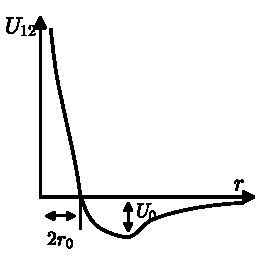
\includegraphics[width=5.5cm]{fig11.pdf}\\[0.3em]{\small 图 11}\end{minipage}\par\nopagebreak

在多原子气体的情形下，相互作用能具有类似的性质，当然，因为它是一个多变量的函数，它已经不可能表示为图 11 所示曲线的形式.

关于函数 $U_{12}$ 的性质的这些知识，足够用来确定在高温和低温两种极限情形下 $B(T)$ 的符号.在高温（$T\gg U_0$）下，在 $r>2r_0$ 的整个区域内我们有 $\dfrac{|U_{12}|}{T}\ll1$，因而在(74.5) $B(T)$ 中的被积式接近于零.因此积分值基本上取决于 $r<2r_0$ 的区域，在这个区域内 $\dfrac{U_{12}}{T}$ 是正的而且很大；所以，在这个区域内被积式是正的，因而整个积分也是正的.由此可见，在高温下 $B(T)$ 是正的.

相反地，在低温（$T\ll U_0$）下，在积分中起主要作用的是 $r>2r_0$ 的区域，在这个区域内 $\dfrac{U_{12}}{T}$ 现在是负的而且绝对值很大.因此在足够低的温度下 $B(T)$ 应该是负的，并且 $B(T)$ 与温度的关系基本上取决于指数因子 $-\exp\left(\dfrac{U_0}{T}\right)$.

因为 $B(T)$ 在高温下是正的而在低温下是负的，所以它应该在某个温度下通过零值\footnote{$B(T_{\mathrm{B}})=0$ 时的温度 $T_{\mathrm{B}}$ 称为\textbf{玻意尔点}. 如果描绘出在给定温度下的 $\dfrac{PV}{T}$ 与 $P$ 的相关曲线，则等温线 $T=T_{\mathrm{B}}$ 在 $P\to0$ 处有水平的切线而且按初始斜率为正和为负分开等温线（所有的等温线都从 $\dfrac{PV}{T}=1$，$P=0$ 的点开始）.}.

最后，我们来研究在非理想气体中发生的焦耳-汤姆孙过程.在这个过程中温度的改变决定于导数
\begin{equation}
  \left(\frac{\partial T}{\partial P}\right)_w
  =\frac{1}{C_p}\left[T\left(\frac{\partial V}{\partial T}\right)_p-V\right]
\end{equation}
（参看(18.2)）.对于理想气体来说，这个导数自然等于 0.对于具有物态方程(74.8)的气体来说，我们得到：
\begin{equation}
  \left(\frac{\partial T}{\partial P}\right)_w
  =\frac{N}{C_p}\left(T\frac{\mathrm{d}B}{\mathrm{d}T}-B\right)
  =\frac{N}{2C_p}\int\left[\mathrm{e}^{-U_{12}/T}
  \left(1-\frac{U_{12}}{T}\right)-1\right]\mathrm{d}V.
\end{equation}

类似于对于 $B(T)$ 所作的讨论那样，不难证明：在高温下应该有 $\left(\dfrac{\partial T}{\partial P}\right)_w<0$，也就是说，在焦耳-汤姆孙过程中，气体从较高的压强过渡到较低的压强时气体的温度升高.而在低温下，$\left(\dfrac{\partial T}{\partial P}\right)_w>0$，也就是说气体的温度随着压强的减小而降低.所以，在每种气体特有的一个温度（反转点）下，焦耳-汤姆孙效应必定反号\footnote{值得注意，我们研究的是弱非理想气体，即压强相对较低. 只在这种近似下，所得到的关于反转温度与压强无关的结果才成立（参看§76习题4）.}.

\begin{xiti}

\noindent{\heiti 习题1}\quad 若气体粒子按照 $U_{12}=\dfrac{\alpha}{r^n}$（$n>3$）的规律相互排斥，试求该气体的 $B(T)$.

解：在(74.5)中把 $\mathrm{d}V$ 写成 $\mathrm{d}V=4\pi r^2\mathrm{d}r$，并对 $\mathrm{d}r$（取积分限从 0 到 $\infty$）进行分部积分；然后用 $\dfrac{\alpha}{Tr^n}=x$ 代入，积分就化为 $\Gamma$ 函数，因而得到：
\begin{equation*}
  B(T)=\frac{2\pi}{3}\left(\frac{\alpha}{T}\right)^{3/n}\Gamma\left(1-\frac{3}{n}\right).
\end{equation*}

\noindent{\heiti 习题2}\quad 在温度和化学势的给定值下，假如气体非常稀薄以致可以认为是理想气体时它该有的压强 $P^{*}$，称为气体的\textbf{逸度}.试求具有热力学势(74.7)的气体的逸度.

解：气体的化学势为（$\mu_{\mathrm{id}}$ 由(42.6)求出）：
\begin{equation*}
  \mu=\mu_{\mathrm{id}}+BP=T\ln P+\chi(T)+BP.
\end{equation*}
按照逸度的定义，令它等同于表达式 $T\ln P^{*}+\chi(T)$，（在具有与(74.7)式同样的精度下）我们得到：
\begin{equation*}
  P^{*}=P\left(1+\frac{BP}{T}\right)=\frac{NT}{V}\left(1+\frac{2NB}{V}\right).
\end{equation*}

\end{xiti}

\section{按密度幂次的展开式}

在上节中所得到的物态方程(74.6)实质上是压强按 $\dfrac{1}{V}$ 幂次的展开式中的头两项：
\begin{equation}
  P=\frac{NT}{V}\left(1+\frac{NB(T)}{V}+\frac{N^2C(T)}{V^2}+\cdots\right).
\end{equation}

展开式的第一项与理想气体相对应，第二项是考虑到一对分子的相互作用时得到的，而以后各项必然涉及三个、四个等多个分子的相互作用\footnote{展开所用的无量纲小参量，实际上是单分子“体积” $v_0$ 与一个分子所占气体体积 $\dfrac{V}{N}$ 之比即 $\dfrac{Nv_0}{V}$.}.

展开式(75.1)中的系数 $B,C,\cdots$ 称为第二、第三、…\textbf{位力系数}.为了确定这些量，从计算势 $\Omega$ 着手比自由能方便.我们仍旧考虑单原子气体，并从普遍公式(35.5)出发，将之应用于同种粒子构成的气体得到：
\begin{equation}
  \mathrm{e}^{-\Omega/T}=\sum_{N=0}^{\infty}\frac{1}{N!}\mathrm{e}^{\mu N/T}
  \int\mathrm{e}^{-E_N(p,q)/T}\,\mathrm{d}\varGamma_N.
\end{equation}

我们引入了因子 $\dfrac{1}{N!}$，之后，积分就可简单地遍及 $N$ 粒子系统的整个相空间取（参看(31.7)）.

在对 $N$ 求和的依次各项中，能量 $E_N(p,q)$ 具有如下的形式.当 $N=0$ 时，当然 $E_0(p,q)\equiv0$.当 $N=1$ 时，它就是一个原子的动能：
\begin{equation*}
  E_1(p,q)=\frac{p^2}{2m}.
\end{equation*}
当 $N=2$ 时，它由两个原子的动能以及它们的相互作用能组成：
\begin{equation*}
  E_2(p,q)=\sum_{a=1}^{2}\frac{p_a^2}{2m}+U_{12}.
\end{equation*}
类似地，
\begin{equation*}
  E_3(p,q)=\sum_{a=1}^{3}\frac{p_a^2}{2m}+U_{123},
\end{equation*}
式中 $U_{123}$ 是三个原子的相互作用能（一般来讲，它不能归结为和式 $U_{12}+U_{13}+U_{23}$）.其余类推.

把这些表达式代入(75.2)，并引进记号
\begin{equation}
  \xi=\frac{\mathrm{e}^{\mu/T}}{(2\pi\hbar)^3}\int\mathrm{e}^{-p^2/2mT}\,\mathrm{d}^3p
  =\left(\frac{mT}{2\pi\hbar^2}\right)^{3/2}\mathrm{e}^{\mu/T}.
\end{equation}

以后我们将看到：这个表达式不是别的，而就是
\begin{equation*}
  \xi=\frac{P_{\mathrm{id}}}{T},
\end{equation*}
式中 $P_{\mathrm{id}}$ 是理想气体在给定的 $T$ 和 $V$ 下的压强.我们得到：
\begin{equation*}
\begin{aligned}
  \Omega=-T\ln\Bigl(1&+\xi V+\frac{\xi^2}{2!}\iint\mathrm{e}^{-U_{12}/T}\,\mathrm{d}V_1\mathrm{d}V_2\\
  &+\frac{\xi^3}{3!}\iiint\mathrm{e}^{-U_{123}/T}\,\mathrm{d}V_1\mathrm{d}V_2\mathrm{d}V_3+\cdots\Bigr).
\end{aligned}
\end{equation*}

$U_{12},U_{123}\cdots$ 中的每一个都只是原子间相对距离的函数；因此，采用原子相对坐标（如相对于第一个原子），积分的重数可降低一次，同时有附加因子 $V$：
\begin{equation*}
\begin{aligned}
  \Omega=-PV=-T\ln\Bigl(1&+\xi V+\frac{\xi^2V}{2!}\int\mathrm{e}^{-U_{12}/T}\,\mathrm{d}V_2\\
  &+\frac{\xi^3V}{3!}\iint\mathrm{e}^{-U_{123}/T}\,\mathrm{d}V_2\mathrm{d}V_3+\cdots\Bigr).
\end{aligned}
\end{equation*}

最后，把这个表达式按 $\xi$ 的幂次展开；所得到的级数可以表示成形式
\begin{equation}
  P=T\sum_{n=1}^{\infty}\frac{J_n}{n!}\xi^n,
\end{equation}
式中
\begin{equation}
\begin{aligned}
  J_1&=1,\qquad J_2=\int\left(\mathrm{e}^{-U_{12}/T}-1\right)\mathrm{d}V_2,\\
  J_3&=\iint\left(\mathrm{e}^{-U_{123}/T}-\mathrm{e}^{-U_{12}/T}
  -\mathrm{e}^{-U_{13}/T}-\mathrm{e}^{-U_{23}/T}+2\right)\mathrm{d}V_2\mathrm{d}V_3
\end{aligned}
\end{equation}
等等.积分 $J_n$ 的构成规则很明显：只有在 $n$ 个原子彼此很接近时，也就是在 $n$ 个原子相互碰撞时，$J_n$ 中的被积式才显著地不等于零.

把(75.4)式对 $\mu$ 求导数，我们就得到气体中的粒子数，因为
\begin{equation*}
  N=-\left(\frac{\partial\Omega}{\partial\mu}\right)_{T,V}
  =V\left(\frac{\partial P}{\partial\mu}\right)_{T,V}.
\end{equation*}
注意到据定义(75.3)有 $\dfrac{\partial\xi}{\partial\mu}=\dfrac{\xi}{T}$，我们得到：
\begin{equation}
  N=V\sum_{n=1}^{\infty}\frac{J_n}{(n-1)!}\xi^n.
\end{equation}

两个方程式(75.4)和(75.6)以参量形式（参量为 $\xi$）确定了 $P,V$ 和 $T$ 之间的联系，即确定了气体的物态方程.从这两个方程式中消去 $\xi$，就得到级数(75.1)形式的物态方程，其项数可以随意定\footnote{在一级近似下，$P=T\xi$，$N=V\xi$，从而 $P=\dfrac{NT}{V}=P_{\mathrm{id}}$. 在二级近似下，
\begin{equation*}
  P=T\xi\left(1+\frac{J_2}{2}\xi\right),\qquad N=V\xi(1+J_2\xi);
\end{equation*}
从这两个等式中消去 $\xi$，（在同样的精确度下）我们得到：
\begin{equation*}
  P=\frac{NT}{V}-\frac{N^2T}{2V^2}J_2,
\end{equation*}
同(74.6)一致.}.

\section{范德瓦尔斯公式}

在气体中分子间的相互作用是非常微弱的.随着相互作用的增强，气体的性质愈来愈偏离理想气体，最后气体变成凝聚体——液体.液体中分子间相互作用很强，并且这种相互作用的性质（从而液体的性质）强烈地依赖于液体的具体类型.由于这种原因，正如以前所指出的，要建立起任何能够定量描述液体性质的普遍公式是不可能的.

但是可以找到某种\textbf{内插公式}来定性地描述液体和气体之间的过渡.这个公式在两种极限情形下应该给出正确的结果.对于稀薄气体，它应化为理想气体适用的公式.随着密度的增加，气体趋近于液体，这时它应该考虑到物质的有限压缩率.于是这样的公式也将定性地描述气体在中间区域内的行为.

为了推导这样的公式，我们更详细地来研究气体在高温下对理想气体的偏离.像前两节一样，我们首先考虑单原子气体；根据与以前相同的理由，所得到的全部公式也同样适用于多原子气体.

对于§74中所描述的一类气体原子间相互作用（图 11），我们有可能确定 $B(T)$ 按倒温度幂次展开的前几项的形式；这里我们将认为比值 $\dfrac{U_0}{T}$ 很小：
\begin{equation}
  \frac{U_0}{T}\ll1.
\end{equation}

注意到 $U_{12}$ 只是原子间距离 $r$ 的函数，在(74.5)的积分中我们可以把 $\mathrm{d}V$ 写成 $\mathrm{d}V=4\pi r^2\mathrm{d}r$.把对 $\mathrm{d}r$ 积分的区域分成两部分，我们写出：
\begin{equation*}
  B(T)=2\pi\int_0^{2r_0}\left(1-\mathrm{e}^{-U_{12}/T}\right)r^2\,\mathrm{d}r
  +2\pi\int_{2r_0}^{\infty}\left(1-\mathrm{e}^{-U_{12}/T}\right)r^2\,\mathrm{d}r.
\end{equation*}

但是当 $r$ 的值在 0 和 $2r_0$ 之间时，势能 $U_{12}$ 一般非常大.因此在第一个积分中，$\exp(-U_{12}/T)$ 项同 1 相比可略.于是这个积分等于正的量
\begin{equation*}
  b=\frac{16}{3}\pi r_0^3.
\end{equation*}

（对于单原子气体，如果把 $r_0$ 看成是原子的半径，那么 $b$ 就是原子体积的四倍）.

在第二个积分中，处处有 $\dfrac{|U_{12}|}{T}\ll\dfrac{U_0}{T}\ll1$.因此可以把其中的被积式按 $\dfrac{U_{12}}{T}$ 的幂次展开直至第一个非零项.那么第二个积分变成
\begin{equation*}
  -\frac{2\pi}{T}\int_{2r_0}^{\infty}\left|U_{12}\right|r^2\,\mathrm{d}r=-\frac{2a}{T},
\end{equation*}
式中 $a$ 是正的常数.因此，我们求得：
\begin{equation}
  B(T)=b-\frac{a}{T}.
\end{equation}

把它代入(74.4)和(74.7)，我们求出气体自由能为
\begin{equation}
  F=F_{\mathrm{id}}+\frac{N^2}{V}(bT-a),
\end{equation}
而热力学势为：
\begin{equation}
  \varPhi=\varPhi_{\mathrm{id}}+NP\left(b-\frac{a}{T}\right).
\end{equation}

所求的内插公式可以从公式(76.3)求得，它本身并不满足必要的条件，因为它并没有考虑到有限的气体压缩率.我们把 $F_{\mathrm{id}}$ 的表达式(42.4)代入(76.3)，于是我们得到：
\begin{equation}
  F=Nf(T)-NT\ln\frac{\mathrm{e}}{N}
  -NT\left(\ln V-\frac{Nb}{V}\right)-\frac{N^2a}{V}.
\end{equation}

在推导气体自由能公式(74.4)时，我们假设虽然气体并未稀薄到可以认为是理想气体，但是毕竟还具有足够大的体积（以致可以忽略掉三个及更多分子的碰撞），也就是说分子间距比分子线度一般大得多.可以说，气体的体积 $V$ 在任何情形下都比 $Nb$ 大得多.于是，
\begin{equation*}
  \ln(V-Nb)=\ln V+\ln\left(1-\frac{Nb}{V}\right)\approx\ln V-\frac{Nb}{V}.
\end{equation*}
所以，(76.5)可以写成形式
\begin{equation}
\begin{aligned}
  F&=Nf(T)-NT\ln\frac{\mathrm{e}}{N}(V-Nb)-\frac{N^2a}{V}=\\
  &=F_{\mathrm{id}}-NT\ln\left(1-\frac{Nb}{V}\right)-\frac{N^2a}{V}.
\end{aligned}
\end{equation}

在这样的形式下，这个公式满足上面所提出的条件，因为当 $V$ 很大时，它化为理想气体的自由能公式，而当 $V$ 很小时，它显示出气体不能无限压缩（$V<Nb$ 时对数的宗量变为负）.

知道了自由能，就可以确定气体的压强：
\begin{equation*}
  P=-\frac{\partial F}{\partial V}=\frac{NT}{V-Nb}-\frac{N^2a}{V^2}
\end{equation*}
或
\begin{equation}
  \left(P+\frac{N^2a}{V^2}\right)(V-Nb)=NT.
\end{equation}

这就是所求的内插形式的实际气体物态方程即\textbf{范德瓦尔斯方程}.当然，它仅仅是满足上面所提出要求的无数个可能内插公式中的一个，而可从其中选出一个的任何物理依据并不存在.范德瓦尔斯公式只是最简单的和最方便的一个而已\footnote{在具体应用这个公式时，常数 $a$ 和 $b$ 的值必须适当选取，以使得同实验最为符合. 这时常数 $b$ 即使对单原子气体也已不能认定是分子体积的四倍.}.

从(76.6)可以求得气体的熵：
\begin{equation}
  S=S_{\mathrm{id}}+N\ln\left(1-\frac{Nb}{V}\right),
\end{equation}

然后求得气体的能量 $E=F+TS$：
\begin{equation}
  E=E_{\mathrm{id}}-\frac{N^2a}{V}.
\end{equation}

由此可以看出：范德瓦尔斯气体的热容 $C_v=\left(\dfrac{\partial E}{\partial T}\right)_v$ 与理想气体的热容是一致的，它只与温度有关，特别是，它可以是常数.而热容 $C_p$ 则很容易证明（参看习题1）不仅与温度有关，而且还与体积有关，因而不可能化为常数.

式(76.9)中的第二项相当于气体分子的相互作用能；它自然是负的，因为分子间平均来讲吸引力占主导.

\begin{xiti}

\noindent{\heiti 习题1}\quad 试求由范德瓦尔斯公式所描述的非理想气体的 $C_p-C_v$.

解：借助于公式(16.10)和范德瓦尔斯方程，我们求得：
\begin{equation*}
  C_p-C_v=\frac{N}{1-\dfrac{2Na}{TV^3}(V-Nb)^2}.
\end{equation*}

\noindent{\heiti 习题2}\quad 试求具有常数热容 $C_v$ 的范德瓦尔斯气体的绝热过程方程.

解：把 $S_{\mathrm{id}}=N\ln V+Nc_v\ln T$（略去无关紧要的常数）代入(76.8)，并令 $S$ 等于常数，我们求得关系式
\begin{equation*}
  (V-Nb)T^{c_v}=\text{常数}.
\end{equation*}
它与理想气体相应方程的差别在于以 $V-Nb$ 代替了 $V$.

\noindent{\heiti 习题3}\quad 将上题所述的气体膨胀到真空中去，求体积从 $V_1$ 到 $V_2$ 时的温度改变.

解：当膨胀到真空中去时，气体的能量保持不变.因此从公式(76.9)（其中 $E_{\mathrm{id}}=NC_vT$）求得：
\begin{equation*}
  T_2-T_1=\frac{Na}{C_v}\left(\frac{1}{V_2}-\frac{1}{V_1}\right).
\end{equation*}

\noindent{\heiti 习题4}\quad 对于范德瓦尔斯气体，求焦耳-汤姆孙过程反转点对温度的依赖关系.

解：反转点取决于等式 $\left(\dfrac{\partial T}{\partial V}\right)_p=\dfrac{T}{V}$（参看(74.9)式）.把(76.7)的 $T$ 代入后给出一个方程式，它必须与(76.7)联立求解.由代数计算可得反转点与压强的如下依赖关系：
\begin{equation*}
  T_{\mathrm{inv}}=\frac{2a}{9b}\left(2\pm\sqrt{1-\frac{3b^2}{a}P}\right)^2.
\end{equation*}
在 $P<\dfrac{a}{3b^2}$ 的每一压强下，存在两个反转点，在这两点之间导数 $\left(\dfrac{\partial T}{\partial P}\right)_w$ 为正，而在这个温度区间之外为负.当 $P>\dfrac{a}{3b^2}$ 时，反转点不存在而且处处 $\left(\dfrac{\partial T}{\partial P}\right)_w<0$\footnote{在 $P\to0$ 时的上反转点 $T_{\mathrm{inv}}=\dfrac{2a}{b}$ 对应于§74末尾所考虑的情形. 小压强下的气体下反转点可能由于气体凝聚为液体而不存在.}.

\end{xiti}

\section{位力系数与散射振幅的关系}

在§74—§76中计算位力系数时，我们用的是经典统计学，这在实用上是合理的.但是，关于在量子情形下来计算这些系数的问题具有方法论的意义；这样的情形实际上可以出现在足够低温的氦中.现在我们讨论，如何考虑气体粒子偶对相互作用的量子化来计算第二位力系数（E.~Beth，G.~E.~Uhlenbeck，1937）.我们考虑单原子气体，其原子没有电子角动量；由于特别留意氦的情形，为了明确起见，我们还假定原子核没有自旋，原子遵循玻色统计.

在我们感兴趣的近似下，在确定热力学势 $\Omega$ 的公式(35.3)中只要保留对 $N$ 求和的前三项
\begin{equation}
  \Omega=-T\ln\Bigl[1+\sum_n\mathrm{e}^{(\mu-E_{1n})/T}
  +\sum_n\mathrm{e}^{(2\mu-E_{2n})/T}\Bigr].
\end{equation}

在这里 $E_{1n}$ 代表单个原子的能级，而 $E_{2n}$ 代表两个相互作用的原子所构成系统的能级.我们的目的只在于计算由原子直接相互作用而引起的那些热力学量修正项；量子力学交换效应引起的修正项在理想气体中就已经有，决定于公式(56.15)，根据这一公式，第二位力系数的交换部分（在玻色统计的情形下）等于
\begin{equation}
  B_{\mathrm{exch}}=-\frac{1}{2}\left(\frac{\pi\hbar^2}{mT}\right)^{3/2}.
\end{equation}

由此可见，我们的问题归结为计算和式
\begin{equation*}
  Z^{(2)}=\sum_n\exp\frac{2\mu-E_{2n}}{T},
\end{equation*}
并且从中应该减去对于两个无相互作用原子会得到的表达式.

能级 $E_{2n}$ 由两部分组成：两个原子质心运动的动能 $\left(\dfrac{p^2}{4m}\right.$，其中 $\boldsymbol{p}$ 是质心运动动量，$m$ 是原子质量$\left.\right)$，以及它们的相对运动能量.我们用 $\varepsilon$ 记后者；这就是质量为 $\dfrac{m}{2}$（二原子的约化质量）的粒子在有心力场 $U_{12}(r)$（$U_{12}$ 为原子相互作用势能）中运动的能级.质心的运动总是准经典的，用通常的方式对它的坐标和动量积分（参看§42），我们得到：
\begin{equation*}
  Z^{(2)}=V\mathrm{e}^{2\mu/T}\left(\frac{mT}{\pi\hbar^2}\right)^{3/2}\sum\mathrm{e}^{-\varepsilon/T}.
\end{equation*}

如果用 $Z_{\mathrm{int}}$ 表示和式 $Z^{(2)}$ 中与粒子相互作用相关的部分，那么我们就可以把 $\Omega$ 写成形式
\begin{equation*}
  \Omega=\Omega_{\mathrm{id}}-TV\mathrm{e}^{2\mu/T}
  \left(\frac{mT}{\pi\hbar^2}\right)^{3/2}Z_{\mathrm{int}}.
\end{equation*}

把第二项考虑为对第一项的微小增量，并（借助理想气体的化学势公式(45.5)）用 $T,V$ 和 $N$ 来表示它，我们就得到自由能的表达式
\begin{equation*}
  F=F_{\mathrm{id}}-T\frac{8N^2}{V}\left(\frac{\pi\hbar^2}{mT}\right)^{3/2}Z_{\mathrm{int}}.
\end{equation*}

求对 $V$ 的导数，就得到压强，位力系数中我们所感兴趣的由原子相互作用引起的部分等于
\begin{equation}
  B_{\mathrm{int}}(T)=-8\left(\frac{\pi\hbar^2}{mT}\right)^{3/2}Z_{\mathrm{int}}.
\end{equation}

能级 $\varepsilon$ 的谱由负值的离散谱（对应于原子的有限相对运动）和正值的连续谱（无限运动）组成.前者我们用 $\varepsilon_n$ 来代表；后者可以写成 $\dfrac{p^2}{m}$ 的形式，其中 $\boldsymbol{p}$ 是彼此相距很远的原子的相对运动动量.对离散谱的求和
\begin{equation*}
  \sum_n\mathrm{e}^{|\varepsilon_n|/T}
\end{equation*}
整个包含在 $Z_{\mathrm{int}}$ 内.而对连续谱的积分中必须把对应于无相互作用粒子的自由运动的那一部分分离出来.为此，我们采用以下的方法.

轨道角动量为 $l$ 且有正能量 $\dfrac{p^2}{m}$ 的定态波函数在距离 $r$ 很大时具有渐近形式
\begin{equation*}
  \psi=\frac{\text{常数}}{r}\sin\left(\frac{p}{\hbar}r-\frac{l\pi}{2}+\delta_l\right),
\end{equation*}
式中相移 $\delta_l=\delta_l(p)$ 依赖于势场 $U_{12}(r)$ 的具体形式（参看本教程第三卷§33）.我们形式地假定：距离 $r$ 的变化区域限制在一个很大的但有限的数值 $R$ 以内.

于是动量 $p$ 只能取一系列离散的值，它们由要求当 $r=R$ 时，$\psi$ 变为 0 的边界条件予以确定：
\begin{equation*}
  \frac{p}{\hbar}R-\frac{l\pi}{2}+\delta_l=s\pi,
\end{equation*}
式中 $s$ 是整数.但是当 $R$ 很大时，这一系列 $p$ 值非常稠密，和式
\begin{equation*}
  \sum_p\mathrm{e}^{-p^2/mT}
\end{equation*}
可以变换为积分.为此，将给定 $l$ 的求和项乘以
\begin{equation*}
  \mathrm{d}s=\frac{1}{\pi}\left(\frac{R}{\hbar}+\frac{\mathrm{d}\delta_l}{\mathrm{d}p}\right)\mathrm{d}p,
\end{equation*}
并对 $\mathrm{d}p$ 积分，然后还应该把结果乘以 $2l+1$（轨道角动量取向的简并度），再对 $l$ 求和：
\begin{equation*}
  \sum_p\mathrm{e}^{-p^2/mT}
  =\frac{1}{\pi}\sum_l(2l+1)\int_0^{\infty}
  \left(\frac{R}{\hbar}+\frac{\mathrm{d}\delta_l}{\mathrm{d}p}\right)
  \mathrm{e}^{-p^2/mT}\,\mathrm{d}p.
\end{equation*}

遵循玻色统计且无自旋的粒子，其波函数的坐标部分应该是对称的；这就意味着只允许偶数的 $l$，因此对 $l$ 的求和只对所有偶数求.

自由运动时所有的相移 $\delta_l=0$.因此，$\delta_l=0$ 时仍留下的表达式是和式中与原子相互作用无关的部分，应去除.于是，我们得到所求的 $Z_{\mathrm{int}}$ 的表达式如下：
\begin{equation}
  Z_{\mathrm{int}}=\sum_n\mathrm{e}^{|\varepsilon_n|/T}
  +\frac{1}{\pi}\sum_l\int_0^{\infty}(2l+1)\frac{\mathrm{d}\delta_l}{\mathrm{d}p}\,
  \mathrm{e}^{-p^2/mT}\,\mathrm{d}p,
\end{equation}
而位力系数 $B=B_{\mathrm{exch}}+B_{\mathrm{int}}$ 等于
\begin{equation}
  B(T)=-\frac{1}{2}\left(\frac{\pi\hbar^2}{mT}\right)^{3/2}
  \left(1+16Z_{\mathrm{int}}\right).
\end{equation}

大家知道，势场中运动的粒子的散射振幅据下式由相移 $\delta_l$ 确定\footnote{参看本教程第三卷§123. 进入立体角元 $\mathrm{d}o$ 的散射截面是 $\left|f(\theta)\right|^2\mathrm{d}o$.}：
\begin{equation*}
  f(\theta)=\frac{\hbar}{2\mathrm{i}p}\sum_l(2l+1)
  \left(\mathrm{e}^{2\mathrm{i}\delta_l}-1\right)\mathrm{P}_l(\cos\theta),
\end{equation*}
式中 $\mathrm{P}_l$ 是勒让德多项式，$\theta$ 是入射方向和散射方向之间的夹角；在这里的情形下，求和对所有偶数值 $l$ 求.因而，有可能用散射振幅表示(77.4)中的积分.具体地说，直接把 $f(\theta)$ 的表达式代入，很容易验证有如下的关系式成立：
\begin{equation*}
\begin{aligned}
  \sum_l(2l+1)\frac{\mathrm{d}\delta_l}{\mathrm{d}p}
  ={}&\frac{1}{2\hbar}\frac{\mathrm{d}}{\mathrm{d}p}
  \bigl\{p\left[f(0)+f^{*}(0)\right]\bigr\}+\\
  &+\frac{\mathrm{i}}{4\pi\hbar^2}\int p^2
  \left(f\frac{\partial f^{*}}{\partial p}
  -f^{*}\frac{\partial f}{\partial p}\right)\mathrm{d}o.
\end{aligned}
\end{equation*}

上式左边的和式正好出现在(77.4)的被积式中，将上式代入(77.4)，并对其中一项作分部积分，结果我们得到：
\begin{equation}
\begin{aligned}
  Z_{\mathrm{int}}={}&\sum_n\mathrm{e}^{|\varepsilon_n|/T}
  +\frac{1}{\pi\hbar mT}\int_0^{\infty}p^2\mathrm{e}^{-p^2/mT}
  \left[f(0)+f^{*}(0)\right]\mathrm{d}p+\\
  &+\frac{\mathrm{i}}{(2\pi\hbar)^2}\iint p^2\mathrm{e}^{-p^2/mT}
  \left(f\frac{\partial f^{*}}{\partial p}
  -f^{*}\frac{\partial f}{\partial p}\right)\mathrm{d}p\,\mathrm{d}o.
\end{aligned}
\end{equation}

如果在势场 $U_{12}(r)$ 中具有离散的能级，那么在足够低的温度下 $B(T)$ 对温度的依赖关系基本上决定于对离散能级的求和，这和式随温度的降低而指数增长.但是，离散能级也可能根本不存在；于是位力系数将按幂律而依赖于温度（如果考虑到当 $p\to0$ 时散射振幅趋于一个常数极限，那么很容易证明：在足够低的温度下，$B$ 基本上由 $B_{\mathrm{exch}}$ 这一项所决定）.

应当注意：在相互作用很弱时，粒子间的碰撞可以用玻恩近似描述，这时散射振幅很小，(77.6)式中的第三项是振幅的二次项，可以忽略不计.相互作用很弱时，没有束缚态，因而(77.6)式中的第一项不出现.应用熟知的玻恩近似散射振幅 $f(0)$ 的表达式，容易看出 $F$ 的表达式同(32.3)式（不看二次项）完全一致，这正是在这种情形下理所应当的.

\begin{xiti}

\noindent{\heiti 习题}\quad 试求单原子气体的位力系数 $B(T)$ 在准经典的情形下的量子修正项（数量级为 $\hbar^2$）.

解：对经典自由能的修正由公式(33.15)给出.考虑到这里只出现原子的偶对相互作用，并且 $U_{12}$ 只是原子间距的函数，我们就求得：
\begin{equation*}
  B_{\mathrm{qu}}=\frac{\pi\hbar^2}{6mT^3}\int_0^{\infty}
  \left(\frac{\mathrm{d}U_{12}}{\mathrm{d}r}\right)^2
  \mathrm{e}^{-U_{12}/T}r^2\,\mathrm{d}r.
\end{equation*}
这个表达式就是对公式(74.5)所给出的基本经典值的修正.应当指出：$B_{\mathrm{qu}}>0$.

\end{xiti}

\section{经典等离子体的热力学量}

在§75中所叙述的计算非理想气体热力学量的方法，必定不适于按库仑定律相互作用的带电粒子所组成的气体，因为这时公式中所含的积分发散.所以这样的气体需要特殊处理.

我们考察完全电离的气体（等离子体）.它的粒子的电荷用 $z_ae$ 表示，其中指标 $a$ 用以标识各种不同种类的离子（$e$ 是基本电荷，$z_a$ 是正或负的整数）.另外，设 $n_{a0}$ 是气体单位体积内第 $a$ 种离子的数目.当然，在整体上气体是电中性的，即
\begin{equation}
  \sum_az_an_{a0}=0.
\end{equation}

我们认为气体偏离理想状态不远.为保证这一点，在任何情形下两个离子的平均库仑相互作用能 $\left(-\dfrac{(ze)^2}{r}\right.$，其中 $r\sim n^{-1/3}$ 是离子间距$\left.\right)$ 都必须比离子的平均动能（$\sim T$）小得多.因此，应该有 $(ze)^2n^{1/3}\ll T$，或
\begin{equation}
  n\ll\left(\frac{T}{z^2e^2}\right)^3.
\end{equation}

由于等离子体呈电中性，如果全部粒子彼此独立地均匀分布在空间中，其库仑相互作用能的平均值会是零.因此，等离子体热力学量的一级修正（与它们在理想气体中的值相比）仅仅在考虑了各种粒子位置间的关联之后才会有.为了强调这一点，我们称之为\textbf{关联修正}.

我们首先确定等离子体能量的修正 $E_{\mathrm{corr}}$.从静电学中大家知道，带电粒子系统的电相互作用能可以写成每个电荷与在该电荷处由其余所有电荷所产生势场的乘积之和的一半.在这里
\begin{equation}
  E_{\mathrm{corr}}=V\cdot\frac{1}{2}\sum_aez_an_{a0}\varphi_a,
\end{equation}
式中 $\varphi_a$ 是作用到一个第 $a$ 种离子上的其余电荷的势场.我们以如下方式计算势场\footnote{所述的方法曾被德拜和休克尔用于计算强电解质的热力学量（P.~Debye, E.~Hückel, 1923）.}.

每个离子在其周围产生某种（平均而言是球对称的）不均匀的带电\textbf{离子云}.换而言之，如果在气体中选择某个离子并考虑其余的离子相对于该离子的分布密度，那么这个密度只与离开中心的距离有关.我们用 $n_a$ 表示这个离子云中第 $a$ 种离子的分布密度.每一个第 $a$ 种离子在该给定离子周围电场中的势能是 $z_ae\varphi$，其中 $\varphi$ 是这个场的位势.因此，根据玻尔兹曼公式(38.6)，有
\begin{equation}
  n_a=n_{a0}\exp\left(-\frac{z_ae\varphi}{T}\right).
\end{equation}

常系数已设为 $n_{a0}$，因为离中心很远处（那里 $\varphi\to0$）离子云的密度应该变成气体中的平均离子密度.

离子云的势场与其电荷密度（等于 $\sum ez_an_a$）由静电泊松方程相联系
\begin{equation}
  \Delta\varphi=-4\pi e\sum_az_an_a.
\end{equation}

公式(78.4)和(78.5)一起构成电子和离子的自恰电场方程组.

在我们所作的关于离子相互作用相对微弱的假设下，能量 $ez_a\varphi$ 比 $T$ 小得多，可以把公式(78.4)近似地写成
\begin{equation}
  n_a=n_{a0}-\frac{n_{a0}ez_a}{T}\varphi.
\end{equation}

把这个表达式代入(78.5)并注意到气体整体上为中性的条件(78.1)，就得到方程
\begin{equation}
  \Delta\varphi-\varkappa^2\varphi=0,
\end{equation}
这里引入了记号
\begin{equation}
  \varkappa^2=\frac{4\pi e^2}{T}\sum_an_{a0}z_a^2.
\end{equation}

$\varkappa$ 这个量具有长度倒数的量纲.

方程(78.7)的中心对称解为
\begin{equation*}
  \varphi=\text{常数}\cdot\frac{\mathrm{e}^{-\varkappa r}}{r}.
\end{equation*}

在正中心附近，电场应该变成该电荷（其大小表示为 $z_be$）的纯库仑场.换而言之，对于足够小的 $r$ 应该有 $\varphi\approx ez_b/r$，所以必须取常数 $=z_be$，因此所求的电势分布如下式
\begin{equation}
  \varphi=ez_b\mathrm{e}^{-\varkappa r}/r.
\end{equation}

由此可以顺便指出，在比 $1/\varkappa$ 大得多的距离下，场变得很小.因此，长度 $1/\varkappa$ 可以看成是该离子所产生离子云的线度（它称为\textbf{德拜半径}）.当然，在这里所进行的全部计算都假定这个半径比离子平均间距大很多（显然，该条件与条件(78.2)一致）.

当 $\varkappa r$ 很小时，把电势(78.9)展开成级数，求得
\begin{equation*}
  \varphi=\frac{ez_b}{r}-ez_b\varkappa+\cdots
\end{equation*}

略去的项在 $r=0$ 时为零.第一项是该离子本身的库仑场.第二项显然是离子云中所有其余离子在该离子所在点产生的电势；这也就是应该代入公式(78.3)中去的那个量：$\varphi_a=-ez_a\varkappa$.

因此，我们得到等离子体能量关联部分的如下表达式
\begin{equation}
  E_{\mathrm{corr}}=-\frac{V}{2}\varkappa e^2\sum_an_{a0}z_a^2
  =-Ve^3\sqrt{\frac{\pi}{T}}\Bigl(\sum_an_{a0}z_a^2\Bigr)^{3/2},
\end{equation}
或者，引入气体中各种离子的总数 $N_a=n_{a0}V$ 之后，
\begin{equation}
  E_{\mathrm{corr}}=-e^3\sqrt{\frac{\pi}{TV}}
  \Bigl(\sum_aN_az_a^2\Bigr)^{3/2}.
\end{equation}

这个能量与气体温度的平方根和体积的平方根成反比.

对热力学关系式 $\dfrac{E}{T^2}=-\dfrac{\partial}{\partial T}\dfrac{F}{T}$ 积分，从 $E_{\mathrm{corr}}$ 可以求出自由能的相应增量
\begin{equation}
  F=F_{\mathrm{id}}-\frac{2e^3}{3}\sqrt{\frac{\pi}{TV}}
  \Bigl(\sum_aN_az_a^2\Bigr)^{3/2}
\end{equation}
（必须令积分常数等于 0，因为当 $T\to\infty$ 时应该有 $F=F_{\mathrm{id}}$）.由此得出压强
\begin{equation}
  P=\frac{NT}{V}-\frac{e^3}{3V^{3/2}}\sqrt{\frac{\pi}{T}}
  \Bigl(\sum_aN_az_a^2\Bigr)^{3/2},
\end{equation}
式中 $N=\sum N_a$.借助于小增量定理从 $F$ 可以得到热力学势 $\varPhi$（就像在§74中所做的），也就是把(78.12)中的第二项看成是 $F_{\mathrm{id}}$ 的小增量，并且将之以适当的精度用变量 $P$ 和 $T$ 表示\footnote{这种方法不可用于从(78.11)变换到(78.12)，因为能量(78.11)没有采用这时要求的变量 $S$ 和 $V$ 来表示.}：
\begin{equation}
  \varPhi=\varPhi_{\mathrm{id}}-\frac{2e^3}{3T}\left(\frac{\pi P}{N}\right)^{1/2}
  \Bigl(\sum_aN_az_a^2\Bigr)^{3/2}.
\end{equation}

\section{关联函数方法}

上节所述的德拜-休克尔方法的优点在于物理上简单明了.另一方面，其主要缺点在于不能推广到计算关于浓度的高级近似.因此，我们还要简短地叙述一下由 Н.\,Н.\,博戈留波夫（1946）提出的另一种方法，它虽然比较复杂，但是在原则上可供计算热力学量展开式的后续项.

这种方法以考虑几个原子同时在空间几个给定点位置之间的所谓\textbf{关联函数}为基础.关联函数中最简单也是最重要的是二体关联函数 $w_{ab}$，它正比于同时在空间给定的两点 $\boldsymbol{r}_a$ 和 $\boldsymbol{r}_b$ 发现两个粒子（离子）的概率（两个离子 $a$ 和 $b$ 可以同种，也可以不同种）.由于气体的各向同性和均匀性，这个函数当然只与 $r=\left|\boldsymbol{r}_b-\boldsymbol{r}_a\right|$ 有关.我们适当选取函数 $w_{ab}$ 的归一因子，使得在 $r\to\infty$ 时它趋于 1.

如果函数 $w_{ab}$ 已知，所求的能量 $E_{\mathrm{corr}}$ 可以用如下显而易见的公式积分求出\footnote{当然，该公式本身与粒子相互作用的库仑特征无关，只假定了二体性.}
\begin{equation}
  E_{\mathrm{corr}}=\frac{1}{2V^2}\sum_{a,b}N_aN_b
  \iint u_{ab}w_{ab}\,\mathrm{d}V_a\mathrm{d}V_b,
\end{equation}
式中求和遍及所有种类的离子，而 $u_{ab}$ 是相距为 $r$ 的一对离子的库仑相互作用能.

根据吉布斯分布公式，函数 $w_{ab}$ 由下式给出：
\begin{equation}
  w_{ab}=\frac{1}{V^{N-2}}\int\exp\frac{F-F_{\mathrm{id}}-U}{T}\,
  \mathrm{d}V_1\mathrm{d}V_2\cdots\mathrm{d}V_{N-2},
\end{equation}
式中 $U$ 是所有离子的库仑相互作用能，而积分遍及除两个给定离子以外的所有其余离子的坐标.为了近似计算这个积分，可以利用下面的方法.

把等式(79.2)对离子 $b$ 的坐标求导数，
\begin{equation}
  \frac{\partial w_{ab}}{\partial\boldsymbol{r}_b}
  =-\frac{w_{ab}}{T}\frac{\partial u_{ab}}{\partial\boldsymbol{r}_b}
  -\frac{1}{VT}\sum_cN_c\int\frac{\partial u_{bc}}{\partial\boldsymbol{r}_b}
  w_{abc}\,\mathrm{d}V_c,
\end{equation}
式中后一项的求和遍及离子的所有种类，而 $w_{abc}$ 是三体关联函数，与(79.2)类似，定义如下：
\begin{equation*}
  w_{abc}=\frac{1}{V^{N-3}}\int\exp\frac{F-F_{\mathrm{id}}-U}{T}\,
  \mathrm{d}V_1\mathrm{d}V_2\cdots\mathrm{d}V_{N-3}.
\end{equation*}

假设气体足够稀薄，并且只考虑一级项，就可以用二体关联函数来表示三体关联函数.实际上，忽略去所有三个离子同时相互靠近的可能性，有
\begin{equation*}
  w_{abc}=w_{ab}w_{bc}w_{ac}.
\end{equation*}

在同样的近似下，我们可以认为，即使一对粒子也不会彼此近到使 $w_{ab}$ 明显地与 1 不同.引入小量
\begin{equation}
  \omega_{ab}=w_{ab}-1
\end{equation}
并忽略它们的高次幂，可以写出
\begin{equation}
  w_{abc}=\omega_{ab}+\omega_{bc}+\omega_{ac}+1.
\end{equation}

把该式代入(79.3)右边的积分，只有含 $\omega_{ac}$ 的项留下，其它项由于气体的各向同性而恒等于 0.在(79.3)式右边的第一项中令 $w_{ab}=1$ 已足够.因此，
\begin{equation*}
  \frac{\partial\omega_{ab}}{\partial\boldsymbol{r}_b}
  =-\frac{1}{T}\frac{\partial u_{ab}}{\partial\boldsymbol{r}_b}
  -\frac{1}{TV}\sum_cN_c\int\omega_{ac}
  \frac{\partial u_{bc}}{\partial\boldsymbol{r}_b}\,\mathrm{d}V_c.
\end{equation*}

现在对这个等式的两边取散度，并考虑到
\begin{equation*}
  u_{ab}=\frac{z_az_be^2}{r},\qquad
  \boldsymbol{r}=\boldsymbol{r}_b-\boldsymbol{r}_a,
\end{equation*}
以及熟知的公式
\begin{equation*}
  \Delta\frac{1}{r}=-4\pi\delta(\boldsymbol{r}),
\end{equation*}
由于出现 $\delta$ 函数，后面的积分变得很容易，我们得到
\begin{equation}
  \Delta\omega_{ab}(\boldsymbol{r})=\frac{4\pi z_az_be^2}{T}\,\delta(\boldsymbol{r})
  +\frac{4\pi e^2z_b}{TV}\sum_cN_cz_c\,\omega_{ac}(\boldsymbol{r}).
\end{equation}

可以寻求该方程组如下形式的解
\begin{equation}
  \omega_{ab}(\boldsymbol{r})=z_az_b\omega(\boldsymbol{r}),
\end{equation}
于是方程组化成单一的方程
\begin{equation}
  \Delta\omega(\boldsymbol{r})-\varkappa^2\omega(\boldsymbol{r})
  =\frac{4\pi e^2}{T}\,\delta(\boldsymbol{r}).
\end{equation}

这个最后的方程与德拜-休克尔方法中的方程(78.7)有相同的形式（(79.8)中含有 $\delta$ 函数的一项，相当于加在(78.7)中函数 $\varphi(r)$ 上的在 $r\to0$ 时的边界条件）.方程(79.8)的解为
\begin{equation}
  \omega(\boldsymbol{r})=-\frac{e^2}{T}\frac{\mathrm{e}^{-\varkappa r}}{r},
\end{equation}
它决定等离子体的二体关联函数.

如果计算能量，现在只需把(79.4)、(79.7)、(79.9)中的 $w_{ab}$ 代入(79.1).变换到对两个粒子相对坐标的积分，我们求得
\begin{equation*}
  E_{\mathrm{corr}}=-\frac{V}{2}\sum_{a,b}n_an_b\int_0^{\infty}
  \frac{z_az_be^2}{r}\,\frac{z_az_be^2}{Tr}\,
  \mathrm{e}^{-\varkappa r}\,4\pi r^2\,\mathrm{d}r
\end{equation*}
（由于等离子体的电中性条件，$w_{ab}$ 中的 1 这一项对能量没有贡献）.进行积分后，回到原先的结果(78.11).

在下一级近似中，计算变得很繁.特别是，假设(79.5)现在已不充分，必须引入三体关联函数，它们已经不能化为二体关联函数了.对于它们可得到类似于(79.3)的方程，但现在含有四体关联函数，然而，在给定的（二级）近似下它们可化为三体关联函数\footnote{等离子体热力学量的下一级项，实际上已经由 А.~А.~Веденов（韦杰诺夫）和 А.~И.~Ларкин（拉尔金）（用其它方法）计算了（Веденов А А, Ларкин А И. ЖЭТФ, 1959, 36: 1133.）.}.

\section{简并等离子体的热力学量}

在§78中叙述的理论中假定等离子体远未简并化，即遵循玻尔兹曼统计.现在我们考虑一种情况，等离子体的温度很低，以至于它的电子组分已经简并化：
\begin{equation}
  T\leqslant\frac{\hbar^2}{m}n^{2/3},
\end{equation}
式中 $m$ 是电子质量（参看(57.8)）；但这时由于离子的质量很大，离子组分仍可能远未简并.值得指出，简并等离子体为近理想的条件在于要求
\begin{equation}
  \frac{mz^{2/3}e^2}{\hbar^2n^{1/3}}\ll1
\end{equation}
（参看(57.9)）；等离子体的密度愈高，该条件满足得愈好.对于简并气体而言，（除了温度 $T$ 和体积 $V$ 以外，）方便的变量是它的化学势\footnote{关于混合物组分化学势的定义，参看§85.} $\mu_a$ 而不是粒子数 $N_a$.与此相应，我们将计算关于这些变量的热力学势 $\Omega$.值得注意，这里的化学势并不是各自独立的变量；它们彼此通过由等离子体电中性条件导出的一个关系式相联系：
\begin{equation}
  \sum_az_aN_a=\sum_az_a\frac{\partial\Omega}{\partial\mu_a}=0.
\end{equation}

利用公式
\begin{equation*}
  \left(\frac{\partial\Omega}{\partial\lambda}\right)_{T,V,\mu_a}
  =\left\langle\frac{\partial\hat{H}}{\partial\lambda}\right\rangle,
\end{equation*}
可将 $\Omega$ 对某个参量 $\lambda$ 的导数表示成系统哈密顿算符的相应导数的平均值（参看类似的公式(11.4)，(15.11)）.这里我们取电荷的平方 $e^2$ 作为参量 $\lambda$.等离子体的哈密顿算符含有 $e^2$，它是粒子库仑相互作用算符 $\hat{U}$ 的一个普遍系数.所以
\begin{equation}
  \left(\frac{\partial\Omega}{\partial e^2}\right)_{T,V,\mu_a}
  =\left\langle\frac{\partial\hat{H}}{\partial e^2}\right\rangle
  =\frac{1}{e^2}\left\langle\hat{U}\right\rangle,
\end{equation}
因此计算 $\Omega$ 归结为计算平均值 $\langle\hat{U}\rangle$.

我们将会看到，在近理想简并等离子体中，对理想气体热力学量的修正主要来自电子的电相互作用交换部分（它在经典情况下并不重要，在§78中完全不予考虑）.注意到这一点，我们在算符 $\hat{U}$ 中只写出描述电子库仑相互作用的那些项.

用二次量子化方法计算 $\langle\hat{U}\rangle$ 最为简单.根据这种方法（参看第三卷§64，§65），我们引入归一化的波函数系 $\psi_{p\sigma}$，它描述在体积 $V$ 中运动的动量为 $\boldsymbol{p}$ 且自旋投影为 $\sigma$（$\sigma=\pm\dfrac{1}{2}$）的自由电子状态.动量 $\boldsymbol{p}$ 取无限个离散值，其间距当 $V\to\infty$ 时趋于零.我们再引入电子在 $\psi_{p\sigma}$ 状态中的湮没算符 $\hat{a}_{p\sigma}$ 和产生算符 $\hat{a}^{+}_{p\sigma}$，并借助它们构成 $\psi$ 算符
\begin{equation}
  \hat{\psi}=\sum_{p\sigma}\psi_{p\sigma}\hat{a}_{p\sigma},\qquad
  \hat{\psi}^{*}=\sum_{p\sigma}\psi^{*}_{p\sigma}\hat{a}^{+}_{p\sigma}.
\end{equation}

粒子的库仑相互作用具有“成对”的特征；在二次量子化方法中把这种相互作用算符写成积分的形式
\begin{equation}
  \hat{U}=\frac{1}{2}\iint\hat{\psi}^{+}(\boldsymbol{r}_1)
  \hat{\psi}^{+}(\boldsymbol{r}_2)
  \frac{e^2}{\left|\boldsymbol{r}_1-\boldsymbol{r}_2\right|}
  \hat{\psi}(\boldsymbol{r}_2)\hat{\psi}(\boldsymbol{r}_1)\,
  \mathrm{d}V_1\mathrm{d}V_2.
\end{equation}

对该算符需要做的求平均可分为两步：首先对系统给定的量子态求平均，然后对不同量子态的平衡统计分布求平均.在近理想等离子体中 $\hat{U}$ 起微扰的作用.我们在微扰论的一级近似下，也就是相对于无相互作用的系统即理想气体的状态，计算这个量的平均值.

量子力学求平均归结为求相应的对角矩阵元.把 $\psi$ 算符(80.5)代入后，算符(80.6)被表达成求和形式，其各项为四个产生与湮没算符的各种乘积：
\begin{equation}
  \hat{U}=\frac{1}{2}\sum\left\langle\boldsymbol{p}_1'\boldsymbol{p}_2'\right|U_{12}
  \left|\boldsymbol{p}_1\boldsymbol{p}_2\right\rangle
  \hat{a}^{+}_{p_1\sigma_1}\hat{a}^{+}_{p_2'\sigma_2}
  \hat{a}_{p_2\sigma_2}\hat{a}_{p_1\sigma_1},
\end{equation}
式中求和遍及所有的角动量和自旋分量，而
$\left\langle\boldsymbol{p}_1'\boldsymbol{p}_2'\right|U_{12}
\left|\boldsymbol{p}_1\boldsymbol{p}_2\right\rangle$
是两个电子相互作用能量 $U_{12}=e^2/\left|\boldsymbol{r}_1-\boldsymbol{r}_2\right|$ 的矩阵元；因为库仑相互作用与自旋无关，所以矩阵元对应于电子自旋分量不变的跃迁，即其计算可用纯轨道函数
\begin{equation*}
  \psi_p=\frac{1}{\sqrt{V}}\mathrm{e}^{\mathrm{i}\boldsymbol{p}\cdot\boldsymbol{r}/\hbar}.
\end{equation*}

在和式(80.7)的所有项中，只是那些带有两对指标相同算符 $\hat{a}_{p\sigma}$ 和 $\hat{a}^{+}_{p\sigma}$ 的项才有对角矩阵元并且乘积 $\hat{a}^{+}_{p\sigma}\hat{a}_{p\sigma}$ 可代之以电子在该量子状态的占有数\footnote{至于四个算符有相同指标的乘积项，其项数比之相同指标两对各异的项数极其稀少，因而不必考虑（这样的项对 $\Omega$ 的贡献含有附加因子 $1/V$）.}.令 $\boldsymbol{p}_1=\boldsymbol{p}_1'$，$\boldsymbol{p}_2=\boldsymbol{p}_2'$，得到
\begin{equation}
  \frac{e^2}{2V^2}\sum_{p_1\neq p_2}\sum_{\sigma_1\sigma_2}
  n_{p_1\sigma_1}n_{p_2\sigma_2}
  \int\frac{\mathrm{d}V_1\mathrm{d}V_2}
  {\left|\boldsymbol{r}_1-\boldsymbol{r}_2\right|},
\end{equation}
而令 $\boldsymbol{p}_1'=\boldsymbol{p}_2$，$\boldsymbol{p}_2'=\boldsymbol{p}_1$，$\sigma_1=\sigma_2=\sigma$，得到如下项
\begin{equation}
  -\frac{e^2}{2V^2}\sum_{p_1\neq p_2}\sum_{\sigma}
  n_{p_1\sigma}n_{p_2\sigma}
  \int\mathrm{e}^{\mathrm{i}(\boldsymbol{p}_1-\boldsymbol{p}_2)\cdot
  (\boldsymbol{r}_1-\boldsymbol{r}_2)/\hbar}
  \frac{\mathrm{d}V_1\mathrm{d}V_2}
  {\left|\boldsymbol{r}_1-\boldsymbol{r}_2\right|}
\end{equation}
（这里出现负号是置换算符 $\hat{a}^{+}_{p_1\sigma}$ 和 $\hat{a}_{p_2\sigma}$ 的结果，把乘积
$\hat{a}^{+}_{p_2\sigma}\hat{a}^{+}_{p_1\sigma}\cdot\hat{a}_{p_2\sigma}\hat{a}_{p_1\sigma}$
化为
$\hat{a}^{+}_{p_2\sigma}\hat{a}_{p_2\sigma}\hat{a}^{+}_{p_1\sigma}\hat{a}_{p_1\sigma}$
必须作置换，而费米子的这些算符是反对易的）.

式(80.8)各项是空间均匀分布的电子的直接库仑相互作用能.正如在§78中已经指出的，由于等离子体呈电中性，这些项实际上正好相消，类似于表示其它粒子（离子）彼此间以及与电子间的相互作用能项（也因这缘故(80.8)的积分发散问题不重要）.式(80.9)中诸项含有库仑势的非对角矩阵元，表示要找的交换效应\footnote{为进一步说明(80.8)和(80.9)诸项的结构，我们指出，前者中的同指标算符对 $\hat{a}_{p\sigma},\hat{a}^{+}_{p\sigma}$ 来自同一空间点（$\boldsymbol{r}_1$ 或 $\boldsymbol{r}_2$）的 $\psi$ 算符；而在(80.9)的诸项中它们来自不同点的 $\psi$ 算符.}.

注意到在宏观体积 $V$ 下，电子的动量实际上具有一系列连续值，将对 $\boldsymbol{p}_1,\boldsymbol{p}_2$ 的求和转为对
$\dfrac{V^2}{(2\pi\hbar)^6}\,\mathrm{d}^3p_1\mathrm{d}^3p_2$
的积分（这时 $\boldsymbol{p}_1\neq\boldsymbol{p}_2$ 的限制变得不重要）.(80.9)中的积分等于\footnote{这里用了熟知的库仑势傅里叶分量表示式
\begin{equation*}
  \int\mathrm{e}^{\mathrm{i}\boldsymbol{k}\cdot\boldsymbol{r}}\,\frac{\mathrm{d}V}{r}
  =\frac{4\pi}{k^2}
\end{equation*}
（参看§117习题3的脚注）.}
\begin{equation*}
  V\int\mathrm{e}^{\mathrm{i}(\boldsymbol{p}_1-\boldsymbol{p}_2)\cdot\boldsymbol{r}/\hbar}
  \,\frac{\mathrm{d}V}{r}
  =V\frac{4\pi\hbar^2}{(\boldsymbol{p}_1-\boldsymbol{p}_2)^2}.
\end{equation*}

结果表达式(80.9)取下式
\begin{equation*}
  -2\pi e^2V\sum_{\sigma}\iint
  \frac{n_{p_1\sigma}n_{p_2\sigma}}{(\boldsymbol{p}_1-\boldsymbol{p}_2)^2}
  \,\frac{\mathrm{d}^3p_1\mathrm{d}^3p_2}{(2\pi)^6\hbar^4}.
\end{equation*}

这个表达式的统计平均（在所考虑的近似下）依理想气体的平衡分布进行.由于理想气体粒子在不同量子态下的统计独立性，这时
$\left\langle n_{p_1\sigma}n_{p_2\sigma}\right\rangle
=\bar{n}_{p_1\sigma}\bar{n}_{p_2\sigma}$；而平均值 $\bar{n}_{p\sigma}$
由费米分布公式
$\bar{n}_{p\sigma}=\left[\mathrm{e}^{(\varepsilon-\mu_e)/T}+1\right]^{-1}$
给出（$\mu_e$ 是电子化学势）.最后，因为所得到的表达式只是与 $e^2$ 成正比，所以根据(80.4)它直接给出所求的等离子体热力学势修正：
\begin{equation}
  \Omega_{\mathrm{exch}}=-\frac{4\pi e^2}{\hbar^4}V\iint
  \frac{\bar{n}_{p_1}\bar{n}_{p_2}}{(\boldsymbol{p}_1-\boldsymbol{p}_2)^2}
  \,\frac{\mathrm{d}^3p_1\mathrm{d}^3p_2}{(2\pi)^6}
\end{equation}
（E.~Wigner, F.~Seitz, 1934）.

在电子气强简并极限情况下（$T\ll\hbar^2n^{2/3}/m$），分布 $\bar{n}_p$ 化为阶跃函数（$p\leqslant p_F$ 时，$\bar{n}_p=1$；$p\geqslant p_F$ 时，$\bar{n}_p=0$）.这时计算积分导致结果\footnote{积分
\begin{equation*}
  I=\iint\frac{\mathrm{d}^3p_1\,\mathrm{d}^3p_2}{(\boldsymbol{p}_1-\boldsymbol{p}_2)^2},\qquad p_1,p_2\leqslant p_F,
\end{equation*}
用代换 $\boldsymbol{p}_1-\boldsymbol{p}_2=\boldsymbol{q}$，$(\boldsymbol{p}_1+\boldsymbol{p}_2)/2=\boldsymbol{s}$ 化为区域 $\left|\dfrac{\boldsymbol{s}\pm\boldsymbol{q}}{2}\right|\leqslant p_F$ 上的积分 $I=\iint q^{-2}\,\mathrm{d}^3q\,\mathrm{d}^3s$. 积分 $\int\mathrm{d}^3s$（在给定的 $\boldsymbol{q}$ 下）是球心相距 $q$ 且半径为 $p_F$ 的两球之间所包的体积：
\begin{equation*}
  \int\mathrm{d}^3s=\frac{4\pi}{3}h^2(3p_F-h),\qquad h=p_F-\frac{q}{2}.
\end{equation*}
然后，对 $\mathrm{d}^3q$ 在区域 $0<q<2p_F$ 上积分，得到 $I=4\pi^2p_F^4$.}
\begin{equation}
  \Omega_{\mathrm{exch}}=-V\frac{e^2p_F^4}{4\pi^3\hbar^4}
  =-V\frac{e^2m^2\mu_e^2}{\pi^3\hbar^4}.
\end{equation}

如果根据(57.3)用电子的数密度 $n_e=N_e/V$ 表示其中的化学势，上式给出自由能的修正：
\begin{equation}
  F_{\mathrm{exch}}=-N_e\frac{3^{4/3}}{4\pi^{1/3}}e^2n_e^{1/3}.
\end{equation}

在玻尔兹曼气体的相反极限情形下（$\mu_e<0$，$|\mu_e|\gg T$），由公式(80.10)计算给出\footnote{在这种情形下
\begin{equation*}
  \bar{n}_{p_1}\bar{n}_{p_2}
  =\exp\left(\frac{2\mu_e}{T}-\frac{p_1^2+p_2^2}{2mT}\right)
  =\exp\left(\frac{2\mu_e}{T}-\frac{4s^2+q^2}{4mT}\right),
\end{equation*}
而对 $\mathrm{d}^3s\,\mathrm{d}^3q$ 的积分扩展到 $\boldsymbol{q}$ 和 $\boldsymbol{s}$ 整个空间.}
\begin{equation}
  \Omega_{\mathrm{exch}}=-V\frac{e^2m^2T^2}{4\pi^2\hbar^4}\,
  \mathrm{e}^{2\mu_e/T}
\end{equation}
或者根据(46.1a)用 $n_e$ 表示 $\mu_e$ 给出
\begin{equation}
  F_{\mathrm{exch}}=-V\frac{\pi e^2\hbar^2n_e^2}{2mT}.
\end{equation}

在 $T\sim\mu_e$ 时，交换修正 $F_{\mathrm{exch}}\sim Ve^2n^{4/3}$，而在§78中求得的关联修正
$F_{\mathrm{corr}}\sim\dfrac{Ve^3n^{3/2}}{\sqrt{T}}$；这时根据近理想性条件
\begin{equation*}
  \frac{F_{\mathrm{corr}}}{F_{\mathrm{exch}}}
  \sim\left(\frac{e^2n^{1/3}}{T}\right)^{1/2}\ll1,
\end{equation*}
即电子交换修正实际上是主导项.然而，在温度升高时，$F_{\mathrm{exch}}$ 比 $F_{\mathrm{corr}}$ 减小得更快（在 $T\gg\mu_e$ 时：$F_{\mathrm{exch}}\propto T^{-1}$，而 $F_{\mathrm{corr}}\propto T^{-1/2}$）.所以存在这样的区域，在其中两种修正有同样的数量级.但是在该区域中，等离子体的简并化已经不强，因此经典公式(78.11)—(78.14)可用于关联修正\footnote{尽管如此，计算任意简并程度下的电子关联修正问题仍有方法论上的意义. 这个问题将在本教程的另外一卷（第九卷）中研究.}.

在以上讨论中假定了等离子体的离子组态不仅非简并，而且几乎是理想的，即离子的相互作用能比它们的热能小得多：$n^{1/3}e^2\ll T$\footnote{为简单起见，在这里和下面的估计中令 $z=1$（氢的等离子体）.}.但是如果等离子体的密度不是太大：
\begin{equation}
  \frac{me^2}{\hbar^2}\ll n^{1/3}\ll\frac{e^2M}{\hbar^2}
\end{equation}
（$M$ 是离子质量），那么温度 $T$ 超过离子的简并化温度
\begin{equation}
  T\sim e^2n^{1/3}\gg\frac{\hbar^2n^{2/3}}{M}
\end{equation}
（并且 $T\ll e^4M/\hbar^2$）.在这些条件下离子组分形成非简并的但相当非理想的系统.离子彼此之间及离子与电子之间相互作用能量的最小性这时相应于核的有序配置，即核形成晶格（А.\,А.\,Абрикосов, 1960）.这导致各种粒子的直接库仑相互作用能已经不再完全相抵.在每一个晶胞内离子的场被位于其中的电子所抵消.但是在一个晶胞的范围（其线度 $\sim n^{-1/3}$）内粒子的相互作用能不是零.根据粗略估计，这个能量 $\sim e^2n^{1/3}$，而对于整个晶格（晶胞数 $N\sim Vn$）结合能为
\begin{equation}
  \left|E_{\mathrm{latt}}\right|\sim Ne^2n^{1/3}\sim Ve^2n^{4/3}.
\end{equation}

它在数量级上与等离子体的简并电子组分交换能一致.对于稳定晶格，结合能自然是负的\footnote{晶格结合能的定量计算参看：Абрикосов А А. ЖЭТФ, 1960, 39: 1797.}.
